\section{From local material intervals to a measured-field bound}\label{sec:theory}
\subsection{Physical model and reachable data}
Use $\exp(-{\rm i}\omega t)$, a real background wavenumber $k$, and the electric polarization invariant along the axis of a nonmagnetic cylinder. The scalar field obeys $(\Delta+k^2)E=-k^2\chi E$. The outgoing volume kernel is $k^2 {\rm i}H_0^{(1)}(k|x-y|)/4$ \cite{colton,richmond}. Its cell representation gives, for $n$ material cells, $s$ sources and $p$ receivers,
\begin{equation}
 E=B+GJ,\qquad J=XE,\qquad F(X)=SJ,\qquad X=\diag(\chi_i).
 \label{eq:vie}
\end{equation}
Here $B,J,E$ have $s$ columns and $S\in\C^{p\times n}$. A material is common to all sources. The $p\times s$ observed scattered field is $Y$. We work with the array and error scaling used to form that matrix; independent noises per optimized coherent source are not assumed. Data from any material in the admissible class $\mathcal B$ lie at a distance from $Y$ bounded below by
\begin{equation}
 \delta(\mathcal B;Y)=\inf_{X\in\mathcal B}\|SJ_X-Y\|_F.
 \label{eq:distance}
\end{equation}
For an error allowance $r$ a lower endpoint above $r$ rules out $\mathcal B$. Conversely, a single material in $\mathcal B$ with verified residual at most $r$ establishes compatibility. All physically admissible forward states are included if uniqueness of the forward equation is not assumed.

For a real interval at cell $i$ put $m_i=(u_i+\ell_i)/2$, $h_i=(u_i-\ell_i)/2$, $M=\diag(m_i)$, $D_h=\diag(h_i)$. Set $q=J-ME$. The scalar material equation gives $q_i=(\chi_i-m_i)e_i$ for the two row vectors. For real diagonal $W\succeq0,V=V^*$ put $A=D_h W D_h$. Then
\begin{equation}
 q^*Wq-E^*AE\preceq0,\qquad \Imag(q^*VE)=0 .
 \label{eq:row}
\end{equation}
Write $\Herm T=(T+T^*)/2$ and $\Imag T=(T-T^*)/(2{\rm i})$. The inequalities follow on multiplication by every coherent source vector. At one cell the two restrictions, with that row alone, recover the real material law in unlifted variables: testing vectors in $\ker e_i$ forces $q_i=z_i e_i$ (or $q_i=0$ if $e_i=0$), the equality makes $z_i$ real, and the inequality gives $|z_i|\le h_i$. Summing over cells is the source of relaxation.

When $I-GM$ is invertible let
\begin{align}
 E_c&=(I-GM)^{-1}B,\quad J_c=ME_c,\nonumber\\
 T&=(I-GM)^{-1}G,\quad P=S(I-MG)^{-1},\quad y=Y-SJ_c .
 \label{eq:shift}
\end{align}
Substitution in \eqref{eq:vie} gives $E=E_c+Tq$, $J=J_c+(I-MG)^{-1}q$, and $SJ-Y=Pq-y$. The order of $G$ and $M$ matters in the incident-field solve. An implementation can work in $J$ directly without inverting the background.

\begin{theorem}[Spatial contrast intervals]\label{th:main}
Set $D=(Pq-y)^*(Pq-y)$. Define
\begin{align}
 K&=P^*P+W-T^*AT+\Imag(VT),\\
 L&=P^*y+T^*AE_c+\tfrac{{\rm i}}{2}VE_c,\qquad C=y^*y-E_c^*AE_c,\\
 \mathcal A&=\begin{pmatrix}K&-L\\-L^*&C\end{pmatrix},\qquad
 P_s=\diag(0_n,I_s). \label{eq:border}
\end{align}
For any $t\ge0$ define $b(t)=[s-\nn(\mathcal A-tP_s)]_+$, where $\nn$ counts strictly negative eigenvalues. Every admissible residual matrix $D$ has at least $b(t)$ eigenvalues at least $t$. In particular
\begin{equation}
 \delta^2(\mathcal B;Y)\ \ge\ \int_0^\infty b(t)\,dt.
 \label{eq:count}
\end{equation}
If $\np(\mathcal A-tP_s)\ge n+j$ then the $j$th largest eigenvalue of $D$ is strictly greater than $t$. A single test therefore excludes $\mathcal B$ when $jt\ge r^2$. When $K$ is nonsingular, put $\nu=\nn(K)$ and $\mathcal H=C-L^*K^{-1}L$. The integral reduces to
\begin{equation}
 \Tail_\nu(\mathcal H)=\sum_{j=\nu+1}^{s}\big[\lambda_j^\downarrow(\mathcal H)\big]_+.
 \label{eq:tail}
\end{equation}
\end{theorem}
\begin{proof}
Adding the nonpositive sector and the zero optical form in \eqref{eq:row} to $D$ gives the quadratic lower matrix $[q;I]^*\mathcal A[q;I]$. The graph $a\mapsto(qa,a)$ is an injective map from $\C^s$. Restriction of a Hermitian form to its range cannot increase the negative index. At least $b(t)$ eigenvalues of $D-tI$ are therefore nonnegative. The span of the $n+j$ largest eigenvectors, with smallest eigenvalue $\gamma>0$, intersects the graph in dimension at least $j$. Since $\|(qa,a)\|\ge\|a\|$, the resulting lower gap $\gamma$ is uniform in $q$. Integrating the eigenvalue counting function and using $D\succeq0$ gives \eqref{eq:count}. Elimination of nonsingular $K$ gives a congruence of $\mathcal A-tP_s$ to $\diag(K,\mathcal H-tI)$ \cite{haynsworth}. Integrating its count yields \eqref{eq:tail}, including ties and $\nu\ge s$.
\end{proof}

At a singular $K$ the exact count has a useful source-space reduction. Let $Z$ span $\ker K$ orthonormally and let $Q$ be an orthonormal basis for $\ker(Z^*L)$. Set $a=\operatorname{rank}(Z^*L)$, $d_0=\dim\ker K-a$ and $H_r=Q^*(C-L^*K^\dagger L)Q$. Then
\[
 n_\pm(\mathcal A-tP_s)=n_\pm(K)+a+n_\pm(H_r-tI).
\]
Eliminate the range of $K$ and take a singular value decomposition of $Z^*L$. The $a$ nonzero singular values couple $a$ null-state coordinates to $a$ source coordinates. This saddle block has $a$ eigenvalues of each sign and a zero source--source block in its inverse. Eliminating it leaves $H_r-tI$ and $d_0$ uncoupled zeros. Hence \eqref{eq:count} equals $\Tail_{\nn(K)}(H_r)$ with $s-a$ source eigenvalues. In the strict positive-count implementation $\np(\mathcal A-tP_s)-n=\np(H_r-tI)-\nn(K)-d_0$. Exact common null directions can be removed before the test. At a mere numerical near-zero such removal requires an independent justification. The singular example in Appendix~\ref{app:tech} exhibits the difference.

In the original current coordinates put $U=I-MG$. The same augmented matrix has blocks
\begin{align}
 K_J&=S^*S+U^*WU-G^*AG+\Imag(VG),\\
 L_J&=S^*Y+U^*WMB+G^*AB+\tfrac{{\rm i}}2VB,\\
 C_J&=Y^*Y+B^*(MWM-A)B. \label{eq:unshifted}
\end{align}
Indeed $q=UJ-MB$. The congruence is block triangular with lower-right block $I_s$, so it preserves the threshold pencil's inertia and, if regular, the source Schur complement. These facts exclude an apparent gain from merely moving the origin of a fixed material hypothesis. The destructive term for a changed interval is quadratic in its true half-width. A fixed cell contributes none of this term; its known value still changes propagation. A strongly resonant background may make $T$ large even for small $h_i$.

\subsection{Nested hypotheses and the convergence radius}
The rows of the sector can be written as $\Herm[(j_i-\ell_i e_i)^*(j_i-u_i e_i)]$. For a fixed midpoint, widening the interval with fixed multipliers subtracts a positive semidefinite matrix from the bordered pencil. For changing midpoints there is a more useful weight rule.
\begin{proposition}[Transport under interval inclusion]\label{th:transport}
Let $I=[m-h,m+h]\subseteq I'=[m'-h',m'+h']$, with $0<h\le h'$. For arbitrary complex row vectors $(j,e)$ put $Q_I=(j-me)^*(j-me)-h^2 e^*e$. Then $(h'/h)Q_I-Q_{I'}\succeq0$. Thus any set of row weights for the parent box yields an equally strong or stronger count on the child by multiplying each sector weight by its own $h'_i/h_i$. Unchanged rows retain their weights. Known fixed cells may instead be eliminated exactly.
\end{proposition}
\begin{proof}
The coefficient matrix in $(j,e)$ has leading entry $\alpha-1$ and determinant
$-\alpha^2 h^2+\alpha(h^2+h'^2-(m-m')^2)-h'^2$. At $\alpha=h'/h$ this is $(h'/h)((h'-h)^2-(m-m')^2)\ge0$. When the chosen ratio $\alpha=h'/h$ equals one, interval inclusion and equal widths imply $I=I'$ and the difference vanishes. Sum the inequalities before performing any elimination. The common optical form in $J$ is unchanged. Eigenvalue ordering then proves the statement also for the direct threshold test.
\end{proof}
This elementary sector calculation permits a branch search to reuse evidence paid for on an ancestor. Taking an unchanged scalar weight on two nonconcentric intervals need not preserve the computed lower endpoint. Excluding an ancestor also excludes its descendants without any new linear algebra.

For width $w$ uniform on an active set with all other cells fixed, $\|wT\|_2<1$ on the active set suffices for a Neumann expansion of $(I-T\Delta)^{-1}$ for every $\|\Delta\|_2\le w$. This yields the comparison bound
\begin{equation}
 \delta\ \ge\ \Big[\|F(M)-Y\|_F-
      \|P\|_2\,w\|E_c\|_F/(1-w\|T\|_2)\Big]_+ .
 \label{eq:neumann}
\end{equation}
The operators in this formula are restricted to the active cells. A directional projection can sharpen the right side. Beyond this norm condition the series may still converge. For example a nilpotent perturbation can have arbitrarily large norm. Failure of the norm test also need not imply negative current inertia: at one cell with $T=2{\rm i},P=3,W=h=1,V=0$, $K=6>0$. To distinguish the mechanisms, we separately test $\rho(wT)$ for an admissible perturbation and count the negative directions of $K$. For nested $\mathcal B_w$, an excluded width and an admitted physical material at a larger width bracket $\inf\{w:\delta(\mathcal B_w;Y)\le r\}$ whenever the domain is regular and attainability is ensured, or bracket the corresponding first-witness width without that extra assumption.
\section{What can be decided before inversion?}\label{sec:use}
\subsection{Linear response, global contrast and losses}
The first Born port map is $A_B x=S\diag(x)B$. A port matrix $Z$ for which
$\Re\langle Z,A_B e_i\rangle_F\le0$ for every cell separates the nonnegative Born cone. Its distance from the measured field is at least $[\Re\langle Z,Y\rangle_F]_+/\|Z\|_F$. This test takes a single inner product after the signs have been checked for the array. Failure of this linear model justifies skipping a terminal Born fit. Nonlinear currents can fit the data for exactly the material whose Born prediction failed.

A second test applies Theorem~\ref{th:main} to $[0,u]^n$. It lower bounds the peak anywhere in the region without assigning a lower endpoint to any particular pixel. On an open two-dimensional domain the Hermitian part of the outgoing volume potential $H_G$ has positive principal symbol $k^2|\xi|^{-2}$. At fixed $k$, fixed bounded region $\Omega$ with boundary of area zero and fixed compact self-adjoint $C_0$, the negative-order Weyl law gives
$\nn(I-uH_G+C_0)\sim k^2|\Omega|u/(4\pi)$ as $u\to\infty$ \cite{ponge}. This describes a continuum spectral obstruction for that family of operators. Usable exterior angular orders instead scale roughly as $2ka$ for a region of circumscribed radius $a$ at fixed tolerance \cite{bucci87,bucci89}. Neither quantity fixes the distance to a measured field. The discrete index is bounded by $n$, and varying frequency, material classes or spatial weights changes the operator.

For a known loss tangent $\chi=(1+{\rm i}t_\ell)x$ with real $x$, translate by $M=(1+{\rm i}t_\ell)\diag(m_i)$. Apply \eqref{eq:row} to $q/(1+{\rm i}t_\ell)$ and $E$. In unrotated coordinates the optical equality is $\Imag(q^*VE)+t_\ell\Herm(q^*VE)=0$. The half-width in the complex plane is $|1+{\rm i}t_\ell|h_i$. For complex disks the modulus sector remains valid. A general rectangle needs its own valid constraints, and a passive lossy medium obeys a one-sided dissipative law. In particular a change about a lossy background can have negative imaginary part. A second, absolute-current inequality is available if $\Im\chi_i/|\chi_i|^2\ge\alpha>0$ on all nonzero cells. With $R=\Imag G$, $M_a=R+\alpha I\succ0$, $J_a=({\rm i}/2)M_a^{-1}B$ and $C_B=B^*M_a^{-1}B/4$, completing the square gives $(J-J_a)^*M_a(J-J_a)\preceq C_B$. Consequently the reachable receiver matrices lie in
\begin{equation}
 SJ_a+(SM_a^{-1}S^*)^{1/2} V_a C_B^{1/2},\qquad \|V_a\|_2\le1 .
 \label{eq:lossy}
\end{equation}
Indeed the least energy at fixed port value is given by the pseudoinverse on the range; the source Gram inequality is equivalent to a contraction \cite{douglas}. One can bound the distance to this set by its support function. These statements use only the declared losses. Real intervals, even signed ones, require no added absorption.

\subsection{A necessary current and an admissible search space}
For a third decision, suppose a real peak class can fit the data. In original coordinates write $V_-^*J=Z_-$, and let $\Lambda_-$ be the positive magnitudes of the negative eigenvalues of $K_J$. With nonsingular $K_J$ let $L_-=V_-^*L_J$ and $H_+=C_J-L_J^*K_{J,+}^\dagger L_J$. Minimizing only the positive square and testing on a source projector $Q$ yields, for $\|SJ-Y\|_F\le r$,
\begin{equation}
 \tr(QH_+)-r^2 \ \le\
 \|\Lambda_-\|_2\,\|Z_-\|_F^2+2\|L_- Q\|_F\|Z_-\|_F .
 \label{eq:norm}
\end{equation}
This gives a lower bound on the norm in the \emph{whole} negative space if the left side is positive. Individual modes need not have positive lower bounds. On six large-domain examples the necessary unweighted norm ranges from 7.65 to 22.00 for the cap one. Positive current that must accompany a chosen negative component can strengthen the estimate, but the improvement on the global material box was small. Appendix~\ref{app:limits} specifies the scope of that observation.

A solver's affine current space $J_d+UZ$ can be tested directly. Substitute it in \eqref{eq:unshifted} using
\[
 K_U=U^*K_JU,\quad L_U=U^*(L_J-K_JJ_d),\quad
 C_U=C_J+J_d^*K_JJ_d-2\Herm(J_d^*L_J).
\]
Theorem~\ref{th:main} holds on the stated space with $n$ replaced by its number of basis columns. Positive distances from this restricted test describe the proposed current space. A short basis alone cannot establish a positive distance for the full physical medium. The fourth decision concerns a complete spatial material neighbourhood, independently of the basis or where an optimizer starts. Excluding it can save a branch-constrained solve. Abandoning every future iterate of an unrestricted solver would additionally require that all those iterates stay in the excluded set.

For the contraction integral equation $\beta J=R(\chi)(\beta E+J)$, with $\beta>0$, $R(x)=\beta x/(\beta+x)$. On pole-free positive intervals,
$\beta j-R(\ell)(\beta e+j)=\beta^2(j-\ell e)/(\beta+\ell)$.
The sector built from both transformed endpoints is the original sector times the positive factor $\beta^4/[(\beta+\ell)(\beta+u)]$. This accounts for its invariance under consistent row reweighting. The inverse distance gives no universal rule for the optimizer's contraction parameter.

\begin{figure}[!htbp]\centering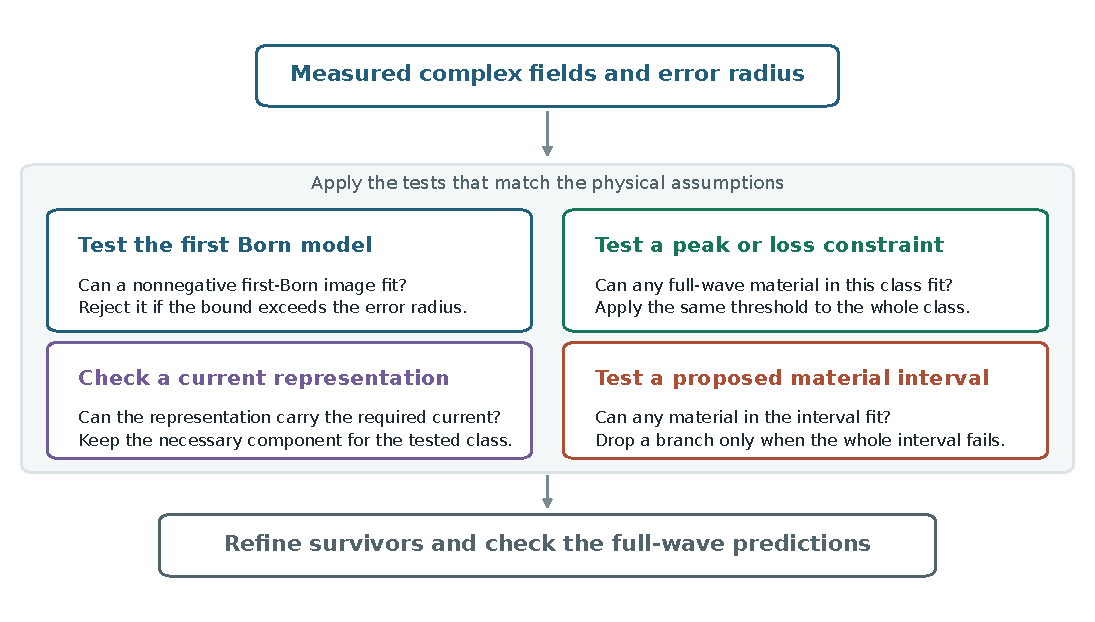
\includegraphics[width=.96\linewidth]{workflow.pdf}
\caption{Four physical decisions available before or alongside inversion. Only a full-wave check of a specified material establishes whether that material explains the observations.}\label{fig:workflow}
\end{figure}

\subsection{Sharing computation between spatial hypotheses}
A fixed array may receive new measurements for many specimens. Let $k_p$ cells change from the baseline interval $[0,b]$ to $[m_i-h_i,m_i+h_i]$ with weights $\alpha_i$ relative to the common sector weight $\mu$. In normalized current units each change adds, in the local rows $(j_i,e_i)$, the Hermitian form
\[
 D_i=\begin{pmatrix}\alpha_i-1&-(\alpha_i m_i-b/2)\\
 -(\alpha_i m_i-b/2)&\alpha_i(m_i^2-h_i^2)\end{pmatrix}.
\]
Thus the change of the \emph{bordered} form has rank at most $2k_p$ even when all $n$ background pixels are unknown. For a positive lower state block $K_b$, stack the pairs $(j_i,e_i)$ in pixel order as $T_p J+e_p$, with a zero in each incident current row and $B_i$ in its field row. Put $D_p=\mathrm{diag}_{\rm blocks}(D_i)$ in this order. In units consistent with $K_b$, let $J_b=K_b^{-1}L_b$, $Z_p=D_p^{-1}+T_pK_b^{-1}T_p^*$, $A_p=T_pJ_b+e_p$. If the inverses exist, completing the square gives
\begin{equation}
 \mathcal H'=\mathcal H_b+A_p^*Z_p^{-1}A_p,\qquad
 \nn(K')=\np(Z_p)-\np(D_p^{-1}) .
 \label{eq:update}
\end{equation}
For the second identity compare the two Schur complements of the matrix with diagonal $K_b,-D_p^{-1}$ and off-diagonal $T_p^*$. The source update follows from stationarity, including the constant $e_p^*D_pe_p$. A singular patch or state can be handled with the bordered count. Our implementation uses a one-sided Fourier floor on the \emph{base} state, then performs \eqref{eq:update} on this lower form; the count refers to that form. It computes the Gram of the patch rows once and retains only the receiver and source dependence in each subsequent test. Perturbative smallness near the high-contrast patch is unnecessary.

The initial geometry calculation includes the original-grid FFT or Green rows and their products. Dense branch algebra then costs order $(2k_p)^3$ per profile and order $(p+s)^2s+s^3$ per reading for the source form; forming the Gram can itself cost order $n k_p^2$ directly. The number and placement of patches are additional inputs. Without small changed supports or repeated geometry this offers no dimensional reduction. It also leaves the cost of discovering candidate material regions untouched.
